\chapter{Regression fits differently than classification}
\label{chap:metrics}

Here we measured whether there is a representation for time in neural activity, based on single-unit recordings on rats' Pre Frontal Cortex. For such, we compared decoding performance in the original data versus in bootstrapped data, which is created by shuffling the time bins of the original data in each trial. If decoding performance on bootstrapped data is equal to the original, then we can infer that the temporal ordering of activity is not essential for decoding, and consequently it is not time that is being decoded. Alternatively, if decoding performance is significantly better in the original activity, then time-ordering is driving decoding performance. 

\section{We can predict elapsed time using the instantaneous firing rate}
    \begin{table}[]
        \centering
        \begin{tabular}{l|rr|rr}
            \hline
            model & \multicolumn{2}{l}{Regression - Bayesian Ridge} & \multicolumn{2}{l}{Classification - LDA} \\
            metric & Explained variance & Pearson's r & Explained variance & Pearson's r \\
            \hline
            bootstrap min  &             -0.000 &      -0.041 &             -1.174 &      -0.036 \\
            bootstrap .025  &             -0.000 &      -0.019 &             -1.069 &      -0.015 \\
            bootstrap .975 &              0.000 &       0.019 &             -0.922 &       0.015 \\
            bootstrap max  &              0.001 &       0.045 &             -0.830 &       0.036 \\
            \hline
            true min  &              0.279 &       0.540 &             -0.186 &       0.453 \\
            true mean &              0.292 &       0.549 &             -0.163 &       0.463 \\
            \hline
        \end{tabular}
        \caption{Bootstrapped versus true decoding performance. The table compares decoding of neural activity when the data is shuffled versus the original. This is shown via comparison of two metrics, Explained variance and Pearson's r, for the two decoding approaches of classification and regression. The upper part of the table shows relevant summary statistics for the bootstrapped data's distribution of results, calculated over 1000 repetitions. The bottom shows relevant statistcs for the true data, calculated over 100 repetitions. The minimum value of performance for the true data is higher than the biggest value for the bootstrapped.}
        \label{tab:bootstrap_time_representation}
    \end{table}
    
    In table \ref{tab:bootstrap_time_representation} we can see that the decoding value for the true data is far from the bootstrapping values. This evidences that the instantaneous firing rate is significantly predictive of the elapsed time. Distinctions between decoding approaches and between the metrics are more thoroughly discussed in the chapter \ref{chap:metrics}. Here we note that the divergence from bootstrapped data is robust to whether we use regression or classification to decode time from the activity. 
    
    \begin{figure}[ht]
        \centering
        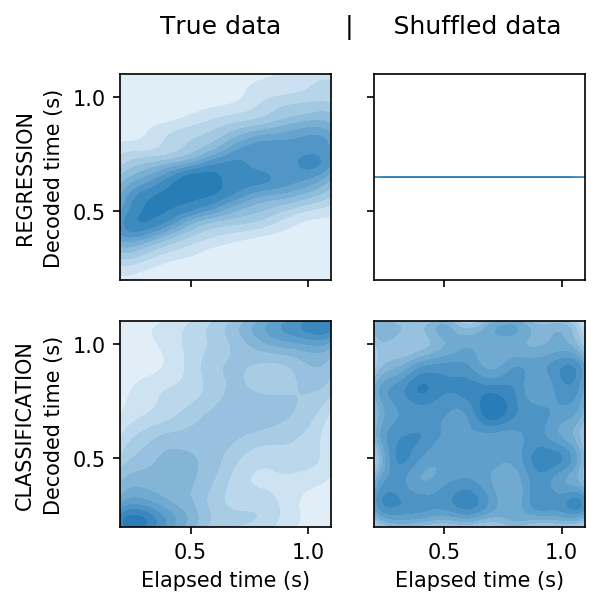
\includegraphics{figures/decoding_kde_bootstrap_vs_true_31.png}
        \caption[Comparison of prediction distributions when data is shuffled]{Comparison of prediction distributions when data is shuffled. Lines refer to the type of algorithm used to assess activity - regression and classification, while columns refer to the type of data - shuffled or not. Darker blues indicate higher density of points. For a given elapsed time, the vertical upon it is the distribution of all predictions calculated over neural activity extracted at that time.}
        \label{fig:decoding_kde_boot}
    \end{figure}
    
    To further assess our decoding results, we look into the distribution of predictions according to the elapsed time of the activity. We can see the full distribution by kernel-density-estimation in figure \ref{fig:decoding_kde_boot}, and a simpler version with mean and variance in figure \ref{fig:decoding_line_boot}. When decoding shuffled data, the regression cannot find information and always predicts the mean, because this minimizes the expected root squared error. This appears in either plot as a single line located at the mean. Classification has no such strategy, because to the classifier there is no "error size" with respect to the predicted class: predicting a .2 and predicting a .9 are equal-sized errors to an example labeled .3. The mean prediction for each time bin, shown in \ref{fig:decoding_line_boot} is located around in the mean value, and distinguishes from the regression results mainly by the huge error bounds. In figure \ref{fig:decoding_kde_boot}, the prediction randomness caused by shuffling is revealed by the multiple density blobs haphazardly located. By repeating the analysis (not shown here), although the other subplots keep the same appearance, the shuffled classification changes considerably, with the blobs in other locations.
    
    \begin{figure}[ht]
        \centering
        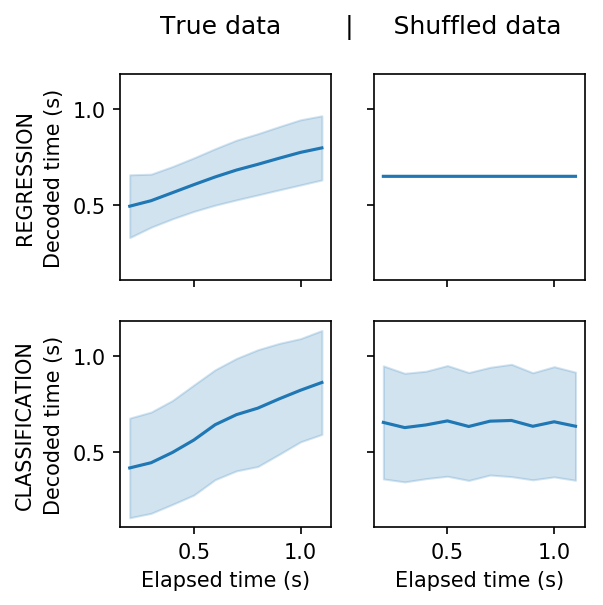
\includegraphics{figures/decoding_line_bootstrap_vs_true_31.png}
        \caption[Summary of prediction distributions comparing when data is shuffled]{Summary of prediction distributions comparing when data is shuffled. Lines refer to the type of algorithm used to assess activity - regression and classification, while columns refer to the type of data - shuffled or not. The darker line is the average decoded value for all data points extracted from a given Elapsed Time. The bands represent the standard deviation around that average.}
        \label{fig:decoding_line_boot}
    \end{figure}
    
    With respect to the true data, we can see in \ref{fig:decoding_line_boot} that the mean prediction has a positive inclination, showing that activity from later in the trial is predicted in average with higher values. While this is seen both in classification and regression, they have distinct patterns of errors, showed in \ref{fig:decoding_kde_boot}, with regression tending towards the mean values while classification tends towards the borders. Anyhow, the positive inclination is indicative of the presence of information in the neural activity, and is consistent with the positive metrics shown in \ref{tab:bootstrap_time_representation}.
